\documentclass[11pt]{article}

\usepackage{url}
\usepackage{multicol}
\usepackage[english]{babel}
\usepackage[margin=1in]{geometry}
\usepackage{graphicx}
\usepackage{subcaption}
\usepackage{enumitem}
\usepackage{amsmath}
\usepackage{amssymb}
\usepackage{wasysym}
\usepackage{color}
\usepackage{float}
\usepackage{nomencl}
\usepackage[title]{appendix}
\makenomenclature
\usepackage{pdfpages}
\usepackage{algorithm}
\usepackage{algpseudocode}
\usepackage{hyperref}
\hypersetup{
    colorlinks=true,
    linkcolor=blue,
    filecolor=magenta,      
    urlcolor=cyan,
    pdftitle={Overleaf Example},
    pdfpagemode=FullScreen,
    }
\title{16-745 Optimal Control Lecture 15}
\author{Reid Graves} 

\begin{document}
\maketitle


\section{Last Time}
\begin{itemize}
    \item Deterministic Optimal Control summary
    \item Linear Quadratic Regulator (LQR) vs. Model Predictive Control (MPC)
    \item Differential Dynamic Programming (DDP) vs. Direct Collocation (DIRCOL)
\end{itemize}

\section{Today}
\begin{itemize}
    \item Optimization with Quaternions
\end{itemize}

\noindent\rule{\textwidth}{0.4pt} % Horizontal line

\section*{Quaternion Recap}

\begin{itemize}
    \item \textbf{4D Unit Vectors}
    \item \textbf{Multiplication Rule}
    
    \begin{equation*}
        q_1 * q_2 = 
        \begin{bmatrix} s_1 \\ v_1 \end{bmatrix} *
        \begin{bmatrix} s_2 \\ v_2 \end{bmatrix} =
        \begin{bmatrix} 
            s_1 s_2 - v_1^T v_2 \\
            s_1 v_2 + s_2 v_1 + v_1 \times v_2
        \end{bmatrix}
    \end{equation*}

    
    \begin{align*}
        L(q_1) &= 
        \begin{bmatrix}
            s_1  & -v_1^T \\
            v_1  & s_1 I + \hat{v}_1
        \end{bmatrix}
        \Rightarrow q_1 * q_2 = L(q_1) q_2
        \\& \hspace{51mm} R(q_2) q_1
    \end{align*}


    \item \textbf{Conjugate}
    
    \begin{equation*}
        q^\dagger = \begin{bmatrix} s \\ -v \end{bmatrix} = T q
   ,\quad
        T = \begin{bmatrix} 1 & 0 \\ 0 & -I \end{bmatrix}
    \end{equation*}

    \item \textbf{Identity}
    
    \begin{equation*}
        q_I = \begin{bmatrix} 1 \\ 0 \end{bmatrix}
    \end{equation*}
    \item ``Hat map" for Quaternions:
    \begin{align*}
        \hat{w} &= \begin{bmatrix}
            0 \\
            \omega
        \end{bmatrix}
        = 
        H\omega, \quad H = \begin{bmatrix}
            0 \\
            I
        \end{bmatrix}
    \end{align*}
\end{itemize}

\section{Geometry of Quaternions}
\begin{figure}[H]
    \centering
    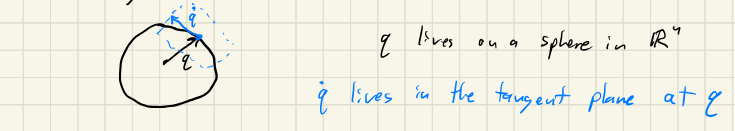
\includegraphics[width=\linewidth]{lecture_15_1.png}
\end{figure}
\begin{itemize}
    \item $q$ lives on a sphere in $\mathbb{R}^4$
    \item $\dot{q}$ lives in the tangent plane at $q$
\end{itemize}

\subsection{Kinematics}
\begin{figure}[H]
    \centering
    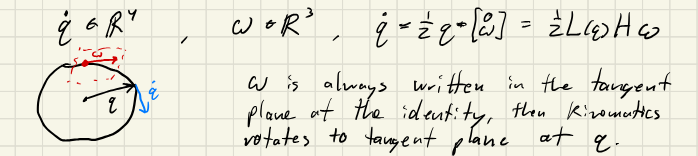
\includegraphics[width=\linewidth]{lecture_15_2.png}
\end{figure}
\begin{align*}
    \dot{q}\in \mathbb{R}^4 \quad,\quad \omega\in \mathbb{R}^3\quad , \quad \dot{q }= \frac{1}{2} q*\begin{bmatrix}
        0 \\ \omega
    \end{bmatrix} = \frac{1}{2}L(q)H\omega
\end{align*}
$\omega$ is always written in the tangent plane at the identity, then kinematics rotates to tangent plane at q.

\subsection{Analogy with unit complex numbers in 2D}
\begin{figure}[H]
    \centering
    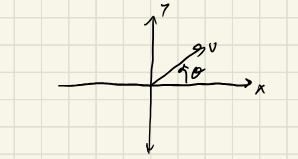
\includegraphics[width=0.5\linewidth]{lecture_15_3.png}
\end{figure}
\begin{align*}
    v &= \cos(\theta) + i \sin(\theta)
    \\
    & \begin{bmatrix}
        \cos(\theta) \\
        \sin(\theta)
    \end{bmatrix}
    \Rightarrow v^Tv = 1
    \\
    \dot{v} &= \frac{\partial v}{\partial \theta}\dot{\theta} = 
    \begin{bmatrix}
        -\sin(\theta) \\
        \cos(\theta)
    \end{bmatrix}
    \dot{\theta}
    =
    \underbrace{
    \begin{bmatrix}
        \cos(\theta) & -\sin(\theta) \\
        \sin(\theta) & \cos(\theta)
    \end{bmatrix}}_{\textcolor{blue}{\text{rotation matrix}}}
    \underbrace{
    \begin{bmatrix}
        0 \\
        \dot{\theta}
    \end{bmatrix}
    }_{\textcolor{blue}{\text{2D ``hat map"}}}
\end{align*}
\begin{figure}[H]
    \centering
    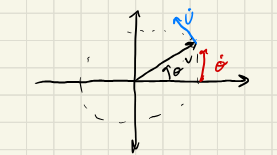
\includegraphics[width=0.5\linewidth]{lecture_15_4.png}
\end{figure}
Kinematics rotates $\dot{\theta}$ from tangent plane at $\theta=0$ to tangent at current $v$

\section{Differentiating Quaternions}

\begin{itemize}
    \item Two key facts
    \begin{enumerate}
        \item Derivatives are really 3D tangent vectors
        \item Rotations compose by multiplication, not addition
    \end{enumerate}
\end{itemize}
\subsection{Infinitessimal Rotation}
\begin{align*}
    \delta q &= \begin{bmatrix}
        \cos\left( \frac{\theta}{2}\right) \\
        a\sin\left(\frac{\theta}{2}\right)
    \end{bmatrix}
    \approx 
    \begin{bmatrix}
        1 \\
        \frac{1}{2}a\theta
    \end{bmatrix}
    \approx
    \underbrace{
    \begin{bmatrix}
        1 \\
        \frac{1}{2}\phi
    \end{bmatrix}
    }_{\textcolor{blue}{\text{small axis-angle vector}}}
    \\
    &= \begin{bmatrix}
        1 \\
        0
    \end{bmatrix}
    +
    \frac{1}{2}
    \begin{bmatrix}
        0 \\
        \phi
    \end{bmatrix}
    =
    \begin{bmatrix}
        1 \\
        0
    \end{bmatrix}
    + \frac{1}{2}H\phi
\end{align*}

\subsection{Compose with q}
\begin{align*}
    q' &= q*\delta q = L(q)\left(
     \begin{bmatrix}
         1 \\
         0
     \end{bmatrix}
     + \frac{1}{2}H\phi
    \right)
    \\
    & \hspace{14mm} = q + \frac{1}{2} \underbrace{L(q)H}_{\textcolor{blue}{G(q) \in \mathbb{R}^{4\times3}}}
    \\
    &\hspace{27mm}\textcolor{blue}{\text{``Attitude Jacobian"}}
\end{align*}
\begin{itemize}
    \item Note: we can use any 3-parameter rotation representation we want for $\phi$. They all linearize the same (up to a permutation/scaling)
    \begin{align*}
        q &= 
        \underbrace{
        \begin{bmatrix}
            \cos\left( \frac{||\phi||}{2} \right)
            \\
            \frac{\phi}{||\phi||}\sin \left( \frac{||\phi||}{2} \right)
        \end{bmatrix}
        }_{\textcolor{blue}{\text{axis-angle}}}
        =
        \underbrace{
        \begin{bmatrix}
            \sqrt{1 - \phi^T\phi}
            \\
            \phi
        \end{bmatrix}
        }_{\textcolor{blue}{\text{vector part of }q}}
        =
        \frac{1}{\sqrt{1 + \phi^T\phi}}
        \underbrace{
        \begin{bmatrix}
            1 \\
            \phi
        \end{bmatrix}
        }_{\textcolor{blue}{\text{Gibbs/Rodriques}}}
    \end{align*}
    \item We'll use the vector part of $q$ in class
    \item This lets us differentiate w.r.t quaternions by inserting $G(q)$ in the right places:
    \begin{align*}
        f(q)& : \underbrace{|\mathbb{H}|}_{\textcolor{blue}{\text{Quaternions (``Hamilton")} }}\rightarrow \mathbb{R} \text{ (Gradient of a scalar-valued function)}
        \\
        \nabla f &= \frac{\partial f}{\partial q}\frac{\partial q}{\partial \phi} = \frac{\partial f}{\partial q}G(q)
        \\
        f(q) &: \mathbb{H}\rightarrow\mathbb{H} \quad\text{ Jacobian of a quaternion-valued function}
        \\
        \phi' &= \underbrace{
        \begin{bmatrix}
            G(f(q))^T\frac{\partial f}{\partial q}G(q)
        \end{bmatrix}
        }_{\textcolor{blue}{\nabla f \in\mathbb{R}^{3\times 3}}}\phi
        \\
        G(f(q))^T&: \textcolor{blue}{\text{transform output}}
        \\
        G(q)&: \textcolor{blue}{\text{transform input}}
    \end{align*}
    \item Hessian of $f(q): \mathbb{H}\rightarrow \mathbb{R}$
    \begin{align*}
        \nabla^2f = G(q)^T\frac{\partial^2 f}{\partial q^2}G(q) + \underbrace{\overbrace{I}^{3\times3}\overbrace{\left( \frac{\partial f}{\partial q}q \right)}^{scalar}}_{\textcolor{blue}{\text{comes from }\frac{\partial G}{\partial q}}}
    \end{align*}
    \item Now we can do Newton's method and DDP and SQP with quaternions
\end{itemize}

\section{Example: Pose Estimation}
\begin{itemize}
    \item Given a bunch of vectors to known landmarks in the environment, determine robot's attitude.
    \item Called ``Wahba's Problem
    \begin{align*}
        \min_q J(q) &= \sum_{k=1}^m ||{^Nx_k} - Q(q) \ ^Bx_k||_2^2 = ||r(q)||_2^2
        \\
        & \hspace{44mm}=r(q)^T\underbrace{r(q)}_{\textcolor{blue}{\text{``residual"}}}
        \\
        ^Nx_k&: \textcolor{blue}{\text{Known vectors in world frame (from map)}}
        \\
        ^Bx_k&: \textcolor{blue}{\text{Observed vectors in body frame (from camera)}}
    \end{align*}
    \item $^Nx_k$ and $^Bx_k$ are unit vectors (``directions")
    \begin{align*}
        r(q) &= 
        \begin{bmatrix}
            ^Nx_1 - Q(q) \ ^Bx_1 \\
            ^Nx_2 - Q(q) \ ^Bx_2 \\
            \vdots \\
            ^Nx_m - Q(q) \ ^Bx_m \\
        \end{bmatrix}
        \Rightarrow \underbrace{\nabla r(q)}_{\textcolor{blue}{3m\times3}} = \underbrace{\frac{\partial r}{\partial q}}_{\textcolor{blue}{3m\times 4}}\underbrace{G(q)}_{\textcolor{blue}{4\times3}}
    \end{align*}
    \item Background: Gauss-Newton for Least-Squares:
    \begin{align*}
        \min_x J(x) &= \frac{1}{2}||R(x)||_2^2 = \frac{1}{2}r(x)^Tr(x)
        \\
        \frac{\partial J}{\partial x} &= r^T(x)\frac{\partial r}{\partial x}
        \\
        \frac{\partial^2 J}{\partial x^2} &= \left(\frac{\partial r}{\partial x}\right)^T\left(\frac{\partial r}{\partial x}\right) + (I\otimes r^T(x))\frac{\partial^2 vec(r)}{\partial x^2}
        \\
        \textcolor{red}{\text{throw this out: }}& (I\otimes r^T(x))\frac{\partial^2 vec(r)}{\partial x^2}
        \\
        \Rightarrow& \left(\frac{\partial J}{\partial x^2}\right)^{-1}\nabla J \approx \begin{bmatrix}
            \left(\frac{\partial r}{\partial x}\right)^T\left(\frac{\partial r}{\partial x}\right)
        \end{bmatrix}^{-1}
        \frac{\partial r}{\partial x}^T r(x)
    \end{align*}
\end{itemize}

\section{Gauss-Newton For Wahba's Problem}
\begin{align*}
    &q\leftarrow q_0\quad\textcolor{blue}{\text{(initial guess)}}
    \\
    &\text{do:}
    \\
    & \quad \nabla r(q) = \frac{\partial r}{\partial q}G(q)
    \\
    & \quad \phi = - \begin{bmatrix}
        (\nabla r^T\nabla r)^{-1}\nabla r^T
    \end{bmatrix}r(q)
    \\
    & \quad q\leftarrow q * \begin{bmatrix}
        \sqrt{1 - \phi^T\phi} \\
        \phi
    \end{bmatrix}
    =L(q) \begin{bmatrix}
        \sqrt{1-\phi^T\phi} \\
        \phi
    \end{bmatrix}
    \\
    &\hspace{40mm}\textcolor{blue}{\text{(multiplicative update)}}
    \\
    &\hspace{20mm}\textcolor{blue}{\text{(in general, do line search)}}
    \\
    & \text{while } ||r(q)|| > \text{tol}
\end{align*}
\end{document}
